\section{Implementation}
\label{sec:implementation}
\begin{figure}[t]
\centering
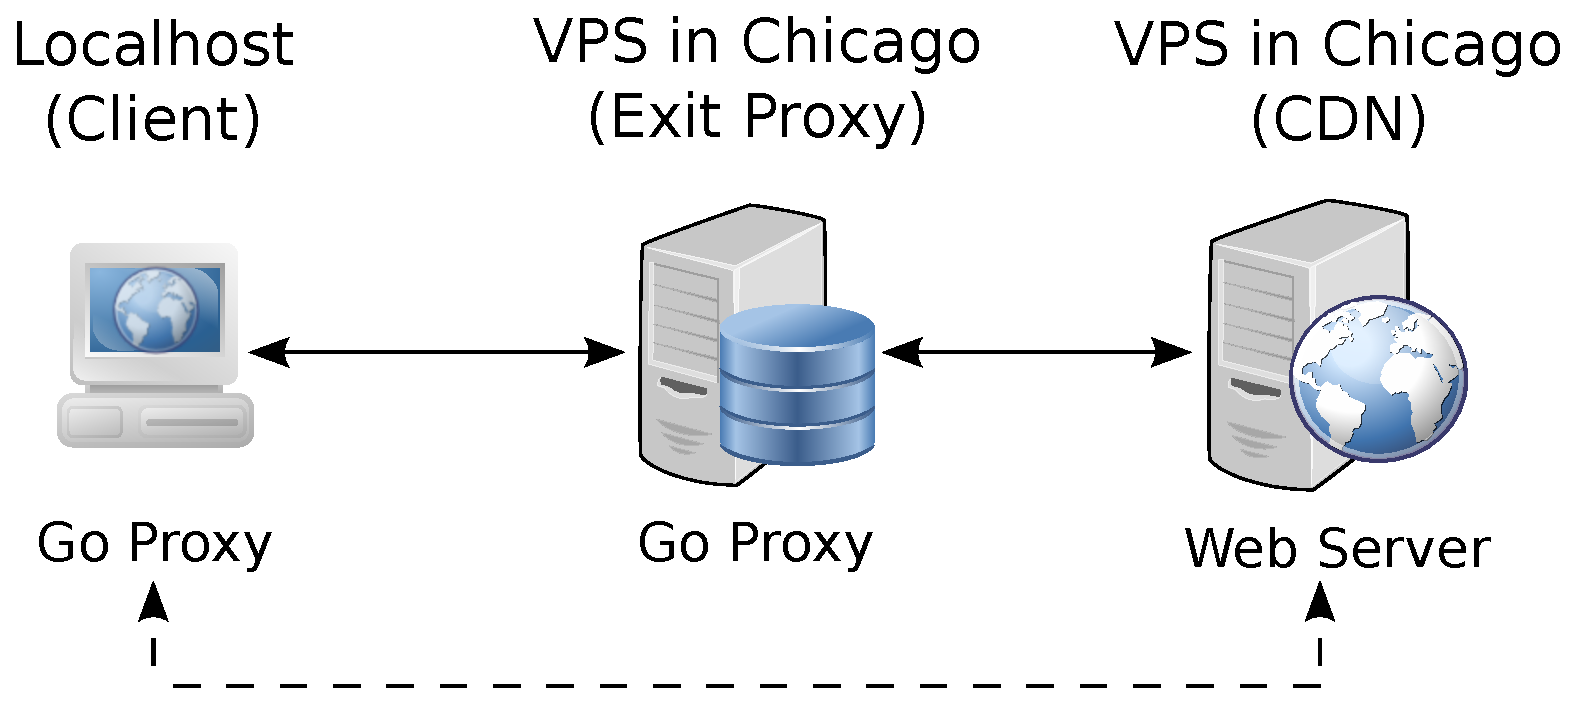
\includegraphics[width=.4\textwidth]{implementation}
\caption{The implementation of our \system{} prototype.  The solid line represents
how \system{} communicates between the components; the dotted line represents how 
a traditional CDN would communicate. $\alpha$ represents the latency between the client 
and the exit proxy; we simulate additional clients on this path by increasing $\alpha$.}
\label{fig:impl}
\end{figure}


\begin{figure*}[t!]
\vspace{-2mm}
  \begin{minipage}[t]{.31\linewidth}
    \centering
     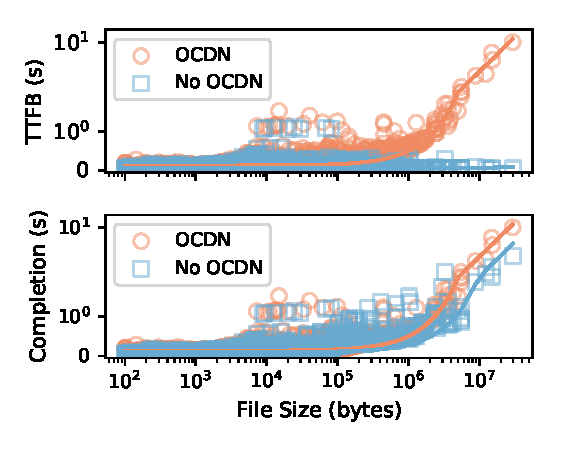
\includegraphics[trim={10 15 10 12},clip,width=\textwidth]{combined}
    \caption{Time to first byte and time to complete a request with and without \system{}.}
    \label{fig:completion}
  \end{minipage}
  \hfill
  \begin{minipage}[t]{.29\linewidth}
    \centering
    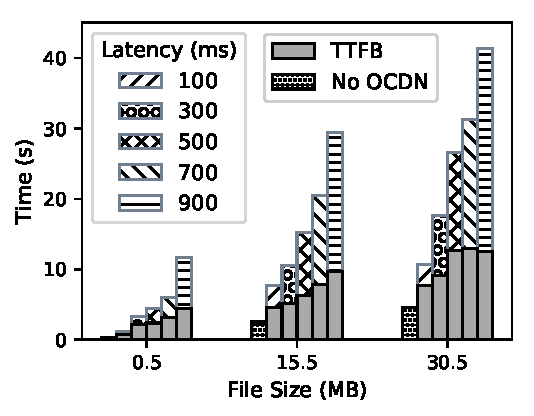
\includegraphics[trim={7 0 10 5},clip,width=\textwidth]{Latency_withoutzero_2}
    %\vspace{-10mm}
    \caption{Time to first byte and time to complete a request with varying the file size and latency.}%; this latency corresponds to $\alpha$ in Figure \ref{fig:impl}.}
    \label{fig:latency}
  \end{minipage}
  \hfill
  \begin{minipage}[t]{.35\linewidth}
    \centering
    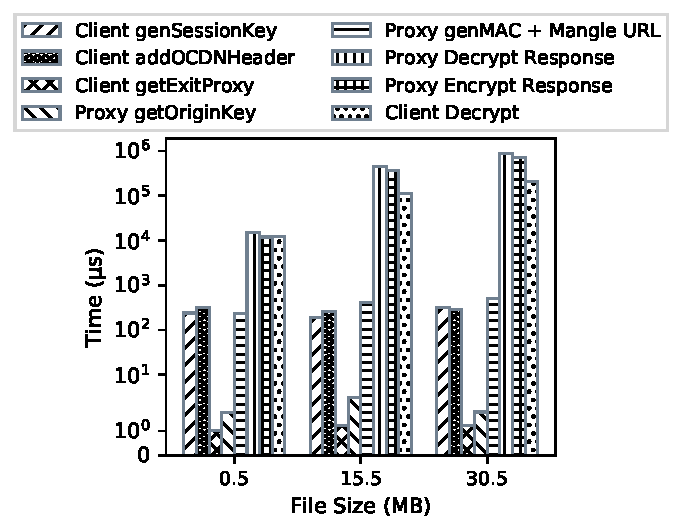
\includegraphics[trim={7 8 7 7},clip,width=\textwidth]{loggrouped_2}
\caption{Overhead of different operations performed by \system{}.}
\label{fig:overhead2}
  \end{minipage}
\end{figure*}


We have implemented a prototype of \system{} to demonstrate its feasibility and 
evaluate its performance.  Our implementation allows a client to send a request 
for content through an exit proxy, which will fetch the corresponding 
encrypted content.  Figure \ref{fig:impl} shows our prototype; the solid line represents
how \system{} communicates between the components, and the dotted line represents how 
a traditional CDN would communicate in our prototype.  Here we will discuss each component---client proxy, exit proxy, 
and CDN---separately, and how they fit together.




\textbf{CDN.} As the design for \system{} requires encrypted content and identifiers
to be stored in the CDN, we cannot request content from real-world CDNs without
establishing a business relationship with an existing CDN ourselves. Additionally,
we must evaluate the performance of \system{} in comparison to the same content, cache locations, etc., so 
we set up a data storage server.  This server is run on a Virtual Private Server
(VPS) located in
Chicago, USA.  To access content, we set up a web server on this VPS machine.  To generate 
plaintext web content, we used Surge~\cite{barford1998generating}, which allows us 
to generate a set of files that are representative of real-world web server file distributions.  
In \system{}, the files are encrypted with a shared key $k$ and the obfuscated file name is the 
HMAC$_{k}$(file name).  We use AES with 256-bit keys for the shared key and SHA-256
for the 
hash function.  Both the plaintext files and encrypted files are stored on this web server, and 
for the purposes of evaluating our prototype, act as a CDN in \system{}.

\textbf{Exit Proxy.} The exit proxy is the component that queries the CDN for
encrypted
content on behalf of a client.  We have implemented a web proxy in Go; this proxy
runs on
a different VPS machine in Chicago, USA.  In addition to proxying web requests, the exit 
proxy also provides cryptographic functionality.  When receiving a request, it rewrites
the URL in the request to be the HMAC$_{k}$(URL), and it parses the headers to retrieve a 
specific header, {\tt X-OCDN}, which contains the client's session key encrypted
under the exit
proxy's public key.  Our implementation uses 2048-bit RSA for asymmetric encryption.  After 
decrypting the session key, it stores it in memory for use on the response.  When 
it receives a response from the CDN, it decrypts the content with the shared key $k$, and 
subsequently encrypts it with the session key (both using AES 256-bit encryption).  The 
exit then forwards the response onto the client proxy.

\textbf{Client Proxy.} The client proxy acts on behalf of the client that is
requesting
content.  This proxy uses the same implementation as the exit proxy, but provides 
different cryptographic functions on the requests and responses.  When a client makes 
a request, the client proxy generates a session key  (AES 256-bit) and looks up the correct exit proxy's 
public key.  The client proxy then adds a header to the request, 
where X-OCDN is the key, the encrypted session key is the value.  The client then forwards this on to the 
exit proxy.  When the client receives a response from the exit proxy, it must decrypt the content 
with the session key it originally generated.   
